\documentclass{beamer}\usepackage[]{graphicx}\usepackage[]{color}
%% maxwidth is the original width if it is less than linewidth
%% otherwise use linewidth (to make sure the graphics do not exceed the margin)
\makeatletter
\def\maxwidth{ %
  \ifdim\Gin@nat@width>\linewidth
    \linewidth
  \else
    \Gin@nat@width
  \fi
}
\makeatother

\definecolor{fgcolor}{rgb}{0.345, 0.345, 0.345}
\newcommand{\hlnum}[1]{\textcolor[rgb]{0.686,0.059,0.569}{#1}}%
\newcommand{\hlstr}[1]{\textcolor[rgb]{0.192,0.494,0.8}{#1}}%
\newcommand{\hlcom}[1]{\textcolor[rgb]{0.678,0.584,0.686}{\textit{#1}}}%
\newcommand{\hlopt}[1]{\textcolor[rgb]{0,0,0}{#1}}%
\newcommand{\hlstd}[1]{\textcolor[rgb]{0.345,0.345,0.345}{#1}}%
\newcommand{\hlkwa}[1]{\textcolor[rgb]{0.161,0.373,0.58}{\textbf{#1}}}%
\newcommand{\hlkwb}[1]{\textcolor[rgb]{0.69,0.353,0.396}{#1}}%
\newcommand{\hlkwc}[1]{\textcolor[rgb]{0.333,0.667,0.333}{#1}}%
\newcommand{\hlkwd}[1]{\textcolor[rgb]{0.737,0.353,0.396}{\textbf{#1}}}%

\usepackage{framed}
\makeatletter
\newenvironment{kframe}{%
 \def\at@end@of@kframe{}%
 \ifinner\ifhmode%
  \def\at@end@of@kframe{\end{minipage}}%
  \begin{minipage}{\columnwidth}%
 \fi\fi%
 \def\FrameCommand##1{\hskip\@totalleftmargin \hskip-\fboxsep
 \colorbox{shadecolor}{##1}\hskip-\fboxsep
     % There is no \\@totalrightmargin, so:
     \hskip-\linewidth \hskip-\@totalleftmargin \hskip\columnwidth}%
 \MakeFramed {\advance\hsize-\width
   \@totalleftmargin\z@ \linewidth\hsize
   \@setminipage}}%
 {\par\unskip\endMakeFramed%
 \at@end@of@kframe}
\makeatother

\definecolor{shadecolor}{rgb}{.97, .97, .97}
\definecolor{messagecolor}{rgb}{0, 0, 0}
\definecolor{warningcolor}{rgb}{1, 0, 1}
\definecolor{errorcolor}{rgb}{1, 0, 0}
\newenvironment{knitrout}{}{} % an empty environment to be redefined in TeX

\usepackage{alltt}
\usepackage{graphicx}
\usepackage{hyperref}
\usepackage{amsmath,amssymb}
\usepackage{algorithm,algpseudocode}
\algdef{SE}[WP]{Wp}{EndWp}[1]{{\bf with prob}\ #1\ }{\algorithmicend\
  {\bf w/prob}}%
\algdef{Ce}[OW]{WP}{Ow}{EndWp}{{\bf otherwise}\ }%
\newcommand{\bx}{\mathbf x}
\newcommand{\bt}{\mathbf t}
\newcommand{\X}{\mathcal X}


\usetheme{Dresden}

\title{evolMC: a package for Monte-Carlo simulation}
\author{W Burchett \and E Roualdes \and G Weyenberg}
\date{Fall 2013}
\IfFileExists{upquote.sty}{\usepackage{upquote}}{}

\begin{document}

\begin{frame}
\maketitle
\end{frame}

\begin{frame}[fragile]
  \frametitle{Getting the package}
  Package {\tt evolMC}.
 
  \url{http://github.com/grady/evol-mc}
\begin{knitrout}
\definecolor{shadecolor}{rgb}{0.969, 0.969, 0.969}\color{fgcolor}\begin{kframe}
\begin{alltt}
\hlkwd{library}\hlstd{(devtools)}
\hlkwd{install_github}\hlstd{(}\hlstr{"evol-mc"}\hlstd{,} \hlstr{"grady"}\hlstd{)}
\hlkwd{library}\hlstd{(evolMC)}
\end{alltt}
\end{kframe}
\end{knitrout}

See the ``example'' package vignette for demo code.
\end{frame}

\begin{frame}
  \frametitle{The Problem}
  \begin{itemize}
  \item We wish to sample from a distribution with multiple modes, separated by regions of very low probability density.

    \item Traditional Metropolis algorithms do not work well here.
      

  \end{itemize}

\begin{center}
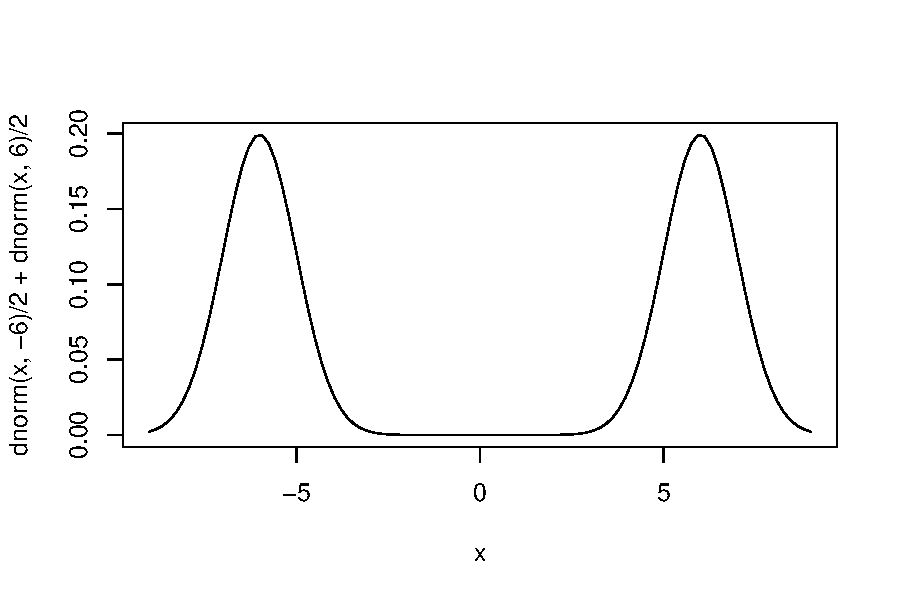
\includegraphics[scale=0.6]{figure/bimodal}  
\end{center}

\end{frame}


\begin{frame}
  \begin{itemize}
  \item Consider a distribution $f(x|t) \propto \exp\{
    -H(x)/t \}$, where $t\ge 1$ is called the \emph{temperature} and
    $H(x)$, called the \emph{fitness function}, corresponds to the
    negative log-density of $x$, up to a constant.
  \item Increasing the temperature causes the distribution to become
    ``flatter'', i.e. to have thicker tails.
    
  \item A \emph{population}
    $\mathbf{x}$ consists of $N$ \emph{individuals} $x_i$, $i = 1,
    \ldots, N$, and we also define an associated set of temperatures
    $\bt = (t_1,\ldots,t_N)$. It is assumed that $x_i \in \mathbb{R}^d$ and the $t_i$
    are in descending order, terminating at the temperature of the
    target distribution. (In most cases this means $t_N =1$.)
  \item Each individual $x_i$ is independently
    sampled from the distribution $f_i(x_i) \propto f(x_i|t_i)$.
  \end{itemize}
\end{frame}

\begin{frame}
\begin{algorithm}[H]
\caption{Evolutionary Monte Carlo}
  \label{alg:emc}
  \footnotesize
  \begin{algorithmic}
    \Procedure{EMC}{}
    \Wp{$p_m$} \Comment{$p_m$ is the \emph{mutation probability}.}
    \State \Call{Mutate}{}
    \Ow 
    \State \Call{Crossover}{}
    \EndWp
    \State  \Call{Exchange}{}
    \EndProcedure
  \end{algorithmic}
\end{algorithm}
\end{frame}

 \begin{frame}
 \begin{algorithm}[H]
   \caption{A Gaussian random-walk {\it mutation}.}
   \label{alg:mutate}
   \footnotesize
   \begin{algorithmic}
     \Procedure{Mutate}{}
     \State Copy the current population to $x$.
     \ForAll{individuals $x_i$ in $x$}
     \State $y \gets \mathcal N_d(x_i,t_i \sigma^2I)$
     \Wp{$\min\{1,\exp(-H(y)/t_i + H(x_i)/t_i)\}$}
     \State $x_i \gets y$
     \EndWp
     \EndFor
     \State Set current population to $x$.
     \EndProcedure
   \end{algorithmic}
 \end{algorithm}
 \end{frame}

\begin{frame}
 \begin{algorithm}[H]
   \caption{The fitness-weighted {\it crossover}.}
   \label{alg:crossover}
   \footnotesize
   \begin{algorithmic}
     \Procedure{Crossover}{}
     \State Copy the current population to $x$.
     \ForAll {individuals $x_i$ in $x$} 
     \State $w_i \gets \exp(-H(x_i))$
     \EndFor
     \State Select $k$ uniformly from $\{1\colon d\}.$
     \State Select $i$ from $\{1\colon N\}$ with weights proportional
     to $\{w_\cdot\}$.
     \State Select $j$ uniformly from $\{1\colon N\} \backslash \{i\}.$ 
    \State In $x$, swap elements $k\colon d$ of individuals $i$ and $j$.
     \Wp {$\cdots$} \Comment{Metropolis update.}
     \State  Set the  current population to $x$.
     \EndWp
     \EndProcedure
   \end{algorithmic}
 \end{algorithm}
 \end{frame}

 \begin{frame}
   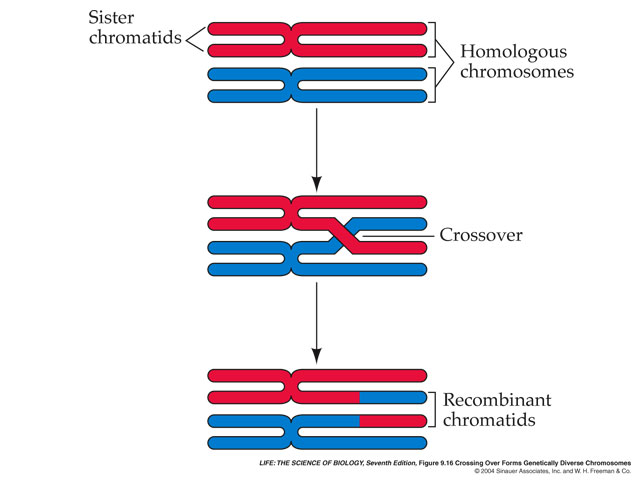
\includegraphics[height=\textheight]{figure/xover}
 \end{frame}
 

\begin{frame}
\begin{algorithm}[H]
\caption{The {\it exchange} attempts to swap individuals between neighboring temperature states.}
  \label{alg:exchange}
  \footnotesize
  \begin{algorithmic}
    \Procedure{Exchange}{}
    \State Copy the current population to $x$.
    \State Select $i$ uniformly from $\{1\colon N\}$. 
    \State Select $j$ uniformly from $\{i\pm 1\}\cap\{1\colon N\}$.
    \State Swap individuals $i,j$ of $x$.
    \Wp{$\min\{1,\exp(-H(x_i)/t_i -H(x_j)/t_j+H(x_i)/t_j + H(x_j)/t_i)\}$}
    \State Set the current population to $x$.
    \EndWp
    \EndProcedure
  \end{algorithmic}
\end{algorithm}
\end{frame}

\end{document}
